\documentclass{beamer}
\usepackage[utf8]{inputenc}

\usetheme{Madrid}
\usecolortheme{default}
\usepackage{amsmath,amssymb,amsfonts,amsthm}
\usepackage{txfonts}
\usepackage{tkz-euclide}
\usepackage{listings}
\usepackage{adjustbox}
\usepackage{array}
\usepackage{tabularx}
\usepackage{gvv}
\usepackage{lmodern}
\usepackage{circuitikz}
\usepackage{tikz}
\usepackage{graphicx}

\setbeamertemplate{page number in head/foot}[totalframenumber]

\usepackage{tcolorbox}
\tcbuselibrary{minted,breakable,xparse,skins}



\definecolor{bg}{gray}{0.95}
\DeclareTCBListing{mintedbox}{O{}m!O{}}{%
  breakable=true,
  listing engine=minted,
  listing only,
  minted language=#2,
  minted style=default,
  minted options={%
    linenos,
    gobble=0,
    breaklines=true,
    breakafter=,,
    fontsize=\small,
    numbersep=8pt,
    #1},
  boxsep=0pt,
  left skip=0pt,
  right skip=0pt,
  left=25pt,
  right=0pt,
  top=3pt,
  bottom=3pt,
  arc=5pt,
  leftrule=0pt,
  rightrule=0pt,
  bottomrule=2pt,

  colback=bg,
  colframe=orange!70,
  enhanced,
  overlay={%
    \begin{tcbclipinterior}
    \fill[orange!20!white] (frame.south west) rectangle ([xshift=20pt]frame.north west);
    \end{tcbclipinterior}},
  #3,
}
\lstset{
    language=C,
    basicstyle=\ttfamily\small,
    keywordstyle=\color{blue},
    stringstyle=\color{orange},
    commentstyle=\color{green!60!black},
    numbers=left,
    numberstyle=\tiny\color{gray},
    breaklines=true,
    showstringspaces=false,
}
%------------------------------------------------------------
%This block of code defines the information to appear in the
%Title page
\title %optional
{2.3.15}
\date{September  2025}
%\subtitle{A short story}

\author % (optional)
{BEERAM MADHURI - EE25BTECH11012}



\begin{document}


\frame{\titlepage}
\begin{frame}{Question}
The scalar product of the vector $\hat{i}+\hat{j}+\hat{k}$ with the unit vector along the sum of vectors $2\hat{i} + 4\hat{j} - 5\hat{k}$ and $\lambda \hat{i} + 2\hat{j} + 3\hat{k}$ is equal to one. Find the value of $\lambda$.
 
\end{frame}
 
\begin{frame}{given data}
 
\text let $\mathbf{A}$, $\mathbf{B}$ and $\mathbf{C}$ be the vectors, such that:
\begin{table}[h!]
    \centering
    \begin{tabular}{|c|c|}
\hline
\textbf{Name} & \textbf{Value} \\ \hline
$\vec{A}$ & $\myvec{2 & 1 \\0 & 3}$ \\ \hline
\end{tabular}

    \caption{Variables used}
    \label{table 2.3.15}
\end{table}
\end{frame}
 
\begin{frame}{solution}
\frametitle{finding Scalar product of $\mathbf{A}$ with unit vector along \vec{B}+ \vec{C}:}
\text given,
\begin{align}
 \frac{\vec{A^\top} (\vec{B}+\vec{C})}{\|\vec{B}+\vec{C}\|} = 1\\
\vec{A^\top} (\vec{B}+\vec{C}) = \|\vec{B}+\vec{C}\|
\end{align}
\text squaring on both sides:
\begin{align}
(\vec{A^\top} (\vec{B}+\vec{C}))^2 = \|\vec{B}+\vec{C}\|^2\\
(\vec{A^\top} \vec{B} + \vec{A^\top} \vec{C})^2 = (\vec{B}+\vec{C})^\top(\vec{B}+\vec{C})
\end{align}
\end{frame}

\begin{frame}
 Substituting the values of \textbf{A},\textbf{B} and \textbf{C}: 
\begin{align}
\left(\begin{pmatrix}1 & 1 & 1\end{pmatrix}  \begin{pmatrix}2 \\4 \\-5\end{pmatrix}+\begin{pmatrix}1 & 1 & 1\end{pmatrix} \begin{pmatrix}\lambda \\2 \\3\end{pmatrix}\right)^2=
\quad\begin{pmatrix}2+\lambda & 6 & -2\end{pmatrix}\begin{pmatrix}2+\lambda \\6 \\-2\end{pmatrix}
\end{align}
\begin{align}
(\lambda+6)^2 = \lambda^2 
+ 4\lambda+44\\
\lambda^2 + 36 + 12\lambda = \lambda^2 + 4\lambda + 44  
\end{align}
\begin{align}8\lambda &= 8 \\\lambda &= 1\end{align}\\
    
Hence value of $\lambda$ is 1.
\end{frame}


\begin{frame}[fragile]
    \frametitle{Python Code}
    \begin{lstlisting}
 import numpy as np
import matplotlib.pyplot as plt
from mpl_toolkits.mplot3d import Axes3D

# --- 1. Define vectors with the calculated lambda = 1 ---
lambda_val = 1
A = np.array([1, 1, 1])
B = np.array([2, 4, -5])
C = np.array([lambda_val, 2, 3])
\end{lstlisting}
\end{frame}

\begin{frame}[fragile]
    \frametitle{Python Code}

    \begin{lstlisting}
# Calculate the resultant vectors ---
# Sum vector S = B + C
S = B + C
# Unit vector s_hat along S
s_hat = S / np.linalg.norm(S)
    \end{lstlisting}
\end{frame}

\begin{frame}[fragile]
    \frametitle{Python Code}

    \begin{lstlisting}
# Set up the 3D plot ---
fig = plt.figure(figsize=(10, 8))
ax = fig.add_subplot(111, projection='3d')
origin = [0, 0, 0]

#  Plot all vectors from the origin ---
ax.quiver(*origin, *A, color='red', label=r'$\vec{A}$')
ax.quiver(*origin, *B, color='blue', label=r'$\vec{B}$')
ax.quiver(*origin, *C, color='green', label=r'$\vec{C}$ (with $\lambda=1$)')
ax.quiver(*origin, *S, color='purple', label=r'Sum Vector $\vec{S} = \vec{B} + \vec{C}$')
ax.quiver(*origin, *s_hat, color='orange', label=r'Unit Vector $\hat{s}$')

    \end{lstlisting}
\end{frame}

\begin{frame}[fragile]
    \frametitle{Python Code}

    \begin{lstlisting}
# Add text labels near the vector tips for clarity ---
ax.text(A[0], A[1], A[2], 'A', color='red', fontsize=12)
ax.text(B[0], B[1], B[2], 'B', color='blue', fontsize=12)
ax.text(C[0], C[1], C[2], 'C', color='green', fontsize=12)
ax.text(S[0], S[1], S[2], 'S', color='purple', fontsize=12)
ax.text(s_hat[0]*1.5, s_hat[1]*1.5, s_hat[2]*1.5, 'ŝ', color='orange', fontsize=14)
\end{lstlisting}
\end{frame}

 
\begin{frame}[fragile]
    \frametitle{Python Code}

    \begin{lstlisting}
# Customize and display the plot ---
ax.set_title('Visualization of Vectors', fontsize=16)
ax.set_xlabel('X-axis')
ax.set_ylabel('Y-axis')
ax.set_zlabel('Z-axis')
ax.set_xlim([-6, 6])
ax.set_ylim([-6, 6])
ax.set_zlim([-6, 6])
ax.legend()
ax.grid(True)
plt.show()
\end{lstlisting}
\end{frame}

\begin{frame}[fragile]
\frametitle{C Code}
\begin{lstlisting}
 #include <stdio.h>
#include <math.h>

/*f(lambda) = (lambda + 6)^2 - (lambda + 2)^2 - 40
  We need f(lambda) = 0 */
double f(double lambda) {
    return (lambda + 6.0)*(lambda + 6.0)
         - (lambda + 2.0)*(lambda + 2.0)
         - 40.0;}
int main(void) {
    double left = -10.0;   // lower bound for search
    double right =  10.0;  // upper bound for search
    double mid;
    double tol = 1e-8;     // desired accuracy
\end{lstlisting}
\end{frame}

\begin{frame}[fragile]
\frametitle{C Code}
\begin{lstlisting}
    // Bisection method
    while ((right - left) > tol) {
        mid = (left + right) / 2.0;
        if (f(mid) == 0.0) break;

        // Root lies where sign changes
        if (f(left) * f(mid) < 0.0)
            right = mid;
        else
            left = mid;
    }
\end{lstlisting}
\end{frame}

\begin{frame}[fragile]
\frametitle{C Code}
\begin{lstlisting}
    double lambda = (left + right) / 2.0;
    printf("Computed value of lambda: %.10f\n", lambda);
 // Optional verification: compute the scalar product
    double sx = lambda + 2.0;
    double sy = 6.0;
    double sz = -2.0;
\end{lstlisting}
\end{frame}

\begin{frame}[fragile]
\frametitle{C Code}
\begin{lstlisting}
    double magnitude = sqrt(sx*sx + sy*sy + sz*sz);
    double scalar_product = (1.0*sx + 1.0*sy + 1.0*sz) / magnitude;
    printf("Verification (scalar product) : %.10f\n", scalar_product);
   return 0;
}
\end{lstlisting}
\end{frame}

\begin{frame}[fragile]
\frametitle{Python and C Code}
\begin{lstlisting}
# File: main.py
import ctypes
import platform
# --- 1. Load the shared library ---
if platform.system() == "Windows":
    lib_path = "./liblambda.dll"
else:
    lib_path = "./liblambda.so"
try:
    lib = ctypes.CDLL(lib_path)
except OSError as e:
    print(f"Error loading library: {e}")
    print("Have you compiled lambda_solver.c?")
    exit()
\end{lstlisting}
\end{frame}

\begin{frame}[fragile]
\frametitle{Python and C Code}
\begin{lstlisting}
# --- 2. Define function signatures ---
# Signature for the first function: solve_for_lambda()
lib.solve_for_lambda.argtypes = [ctypes.c_double, ctypes.c_double, ctypes.c_double]
lib.solve_for_lambda.restype = ctypes.c_double

# Signature for the second function: verify_scalar_product()
lib.verify_scalar_product.argtypes = [ctypes.c_double]
lib.verify_scalar_product.restype = ctypes.c_double
\end{lstlisting}
\end{frame}

\begin{frame}[fragile]
\frametitle{Python and C Code}
\begin{lstlisting}
# --- 3. Prepare input data ---
left_bound = -10.0
right_bound = 10.0
tolerance = 1e-8
# --- 4. Call the C functions ---
# Call the first C function to solve for lambda
computed_lambda = lib.solve_for_lambda(left_bound, right_bound, tolerance)
\end{lstlisting}
\end{frame}

\begin{frame}[fragile]
\frametitle{Python and C Code}
\begin{lstlisting}
# Use the result to call the second C function for verification
scalar_product = lib.verify_scalar_product(computed_lambda)

# --- 5. Print the results ---
print("--- Results from C library ---")
print(f"Computed value of lambda: {computed_lambda:.10f}")
print(f"Verification (scalar product) : {scalar_product:.10f}")

\end{lstlisting}

\end{frame}

\begin{figure}[H]
    \centering
    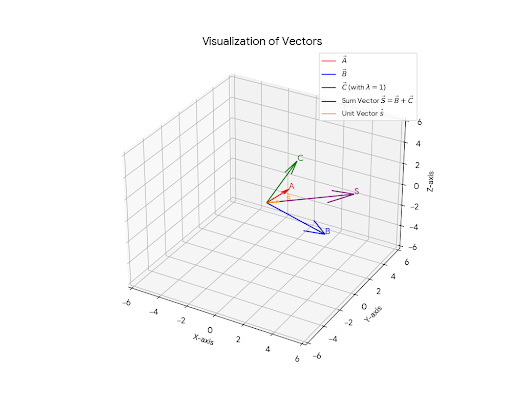
\includegraphics[width=0.7\columnwidth]{Fig.png}
    \caption{Plot}
    \label{fig:placeholder}
\end{figure}


\end{document}